%%test.tex
%\documentclass{article}
%%\usepackage{CJKutf8}
%\usepackage{xeCJK}
%\usepackage{amsmath}
%\usepackage{colortbl}
%\usepackage{graphicx}
%%\begin{CJK}{UTF8}{gbsn}
%%\end{CJK}
%\end{document}
\documentclass{article}
\usepackage{color}
\usepackage{amsmath}
\usepackage{hyperref}
\usepackage[UTF8]{ctex}
\usepackage{graphicx}
\usepackage{xeCJK}
\begin{document}
\title{cuda练习}
\author{师清}
\maketitle
\section{cuda编程模型}
\subsection{异构并行计算}
\noindent
\textcolor{blue}{CPU+GPU}\\
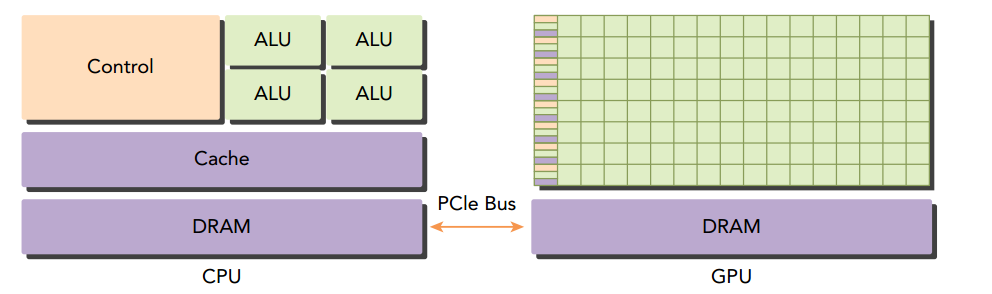
\includegraphics[width=0.9\textwidth]{assets/cpu_gpu.png}\\
Peak computational performance:TFLOPS\\
Memory bandwidth:GB/s\\
\subsection{cuda编程架构}
\noindent
\underline{CUDA: A Platform for Heterogeneous Computing}\\
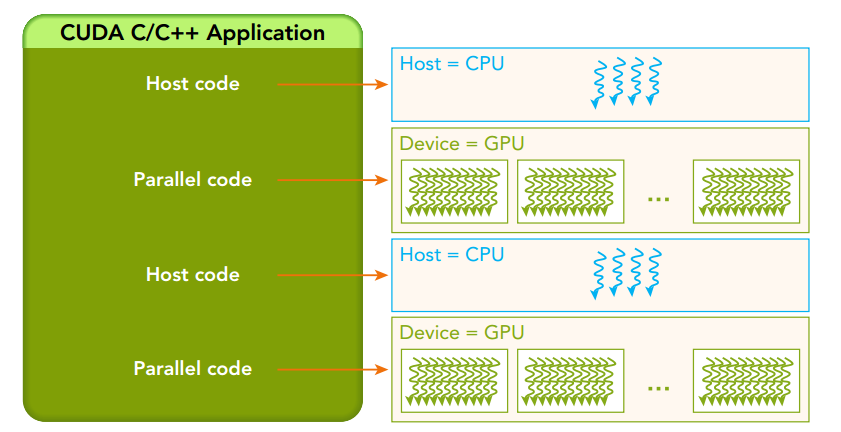
\includegraphics[width=0.9\textwidth]{assets/cuda.png}
\subsubsection{物理上}
\noindent
nvidia gpu架构的演变:\\
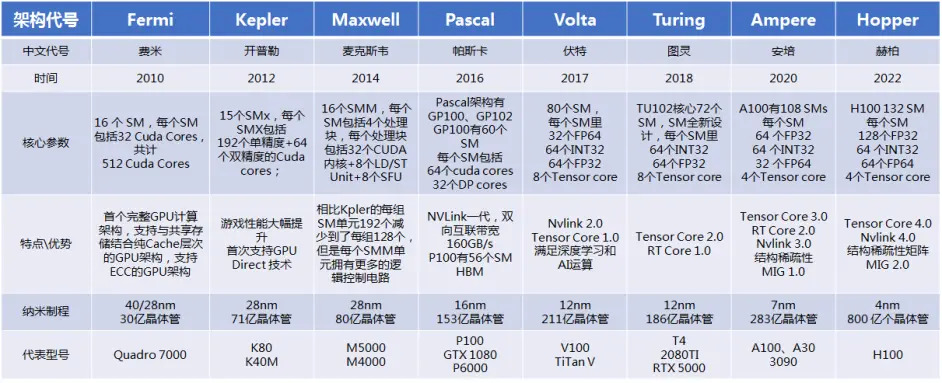
\includegraphics[width=0.9\textwidth]{assets/gpu.jpg}\\
Fermi架构\footnote{\href{https://www.nvidia.com/content/PDF/fermi_white_papers/NVIDIA_Fermi_Compute_Architecture_Whitepaper.pdf}{Fermi架构}}:\\
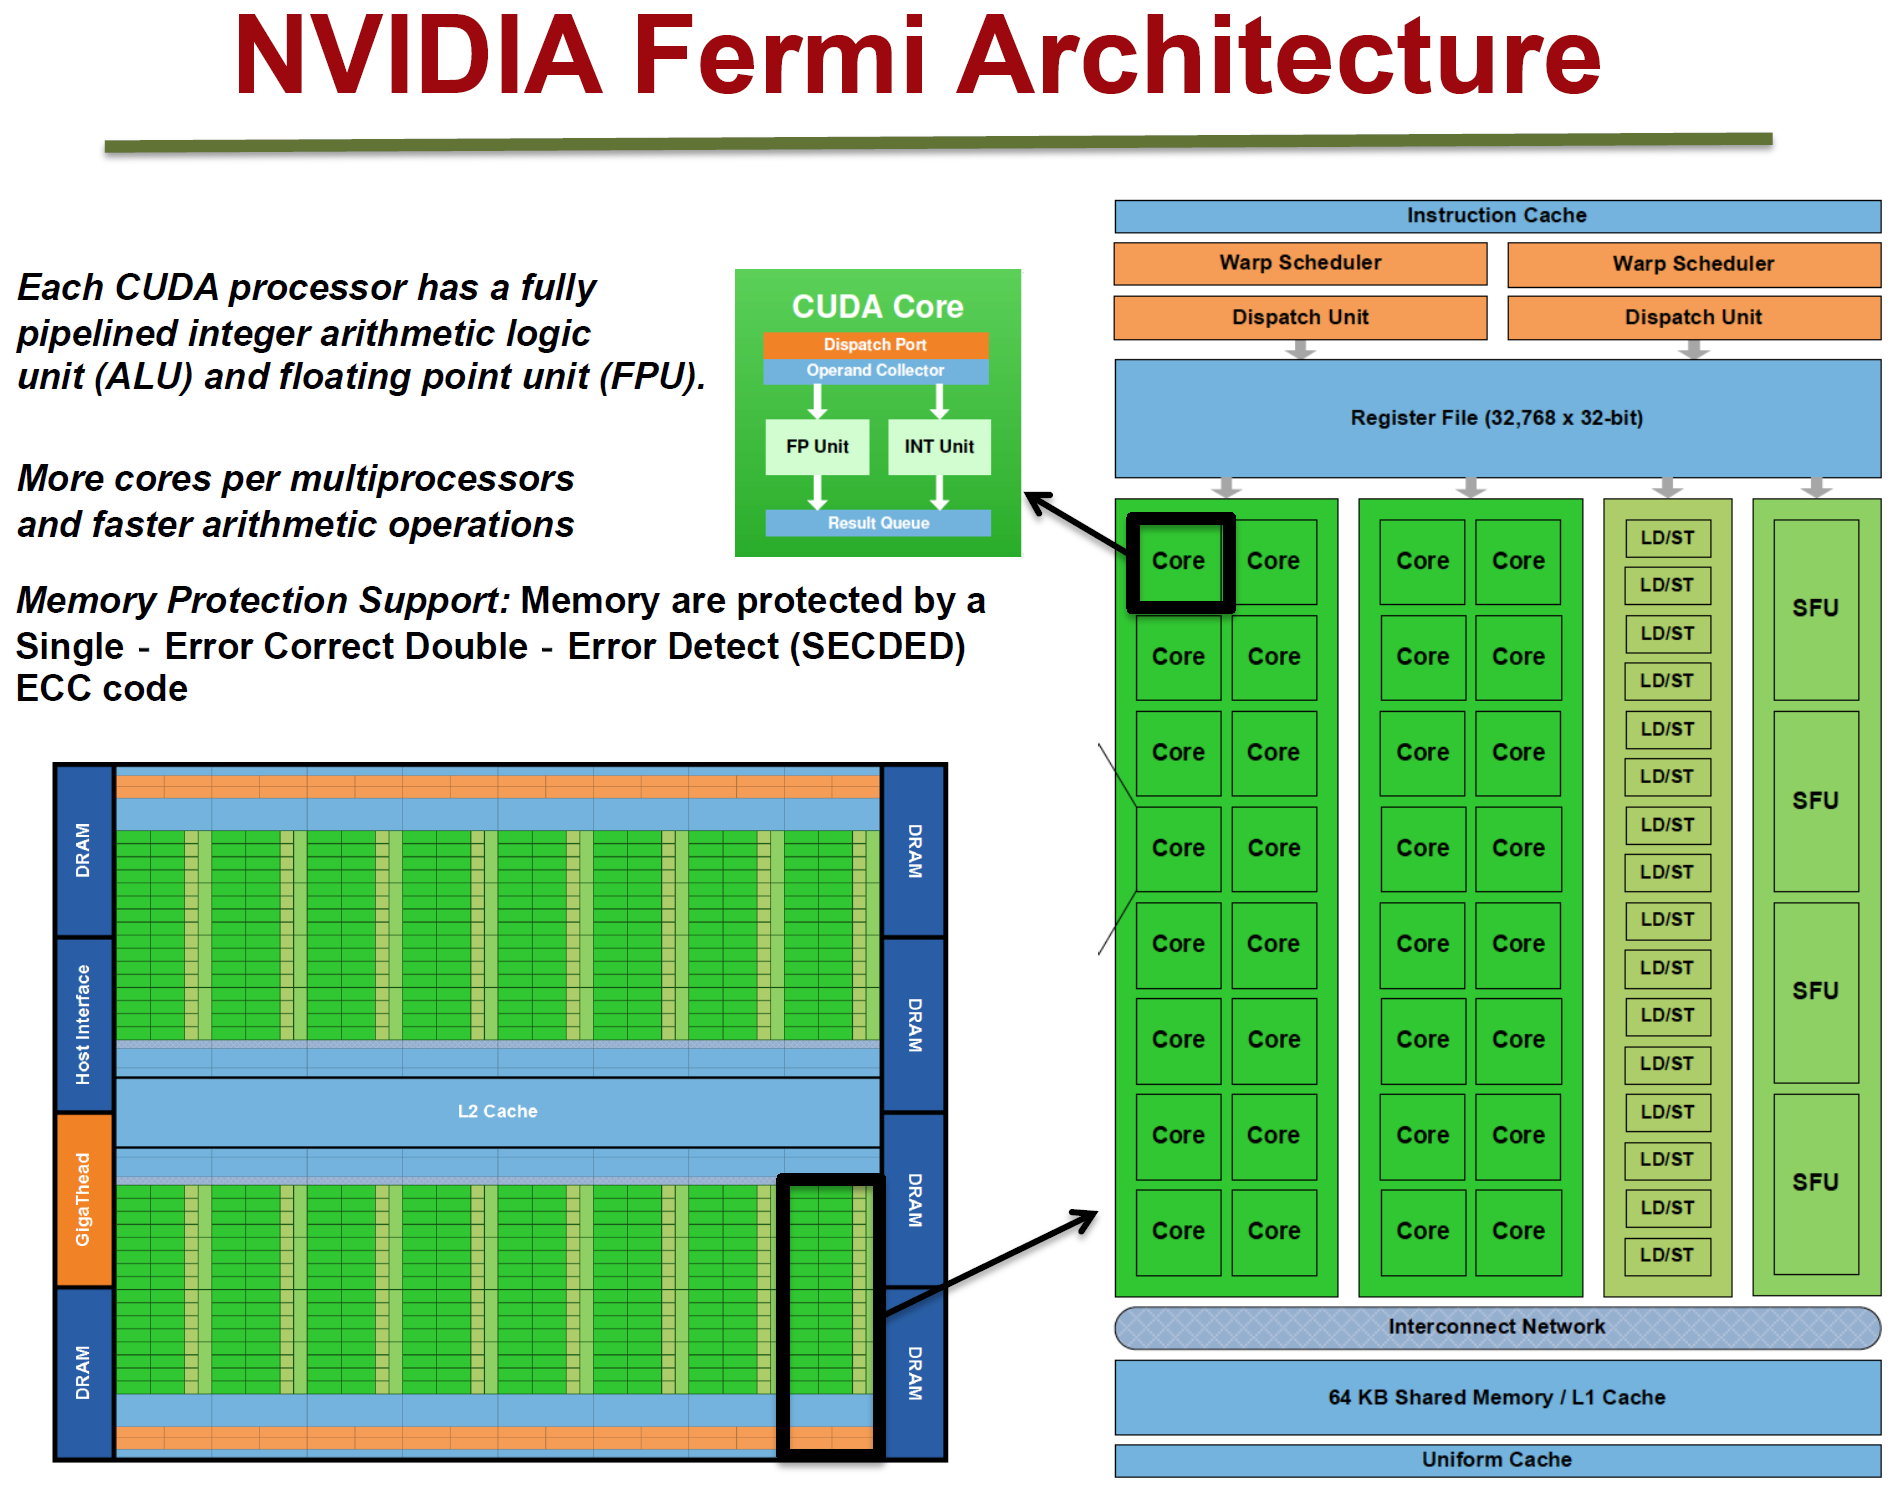
\includegraphics[width=0.9\textwidth]{assets/fermi.png}\\
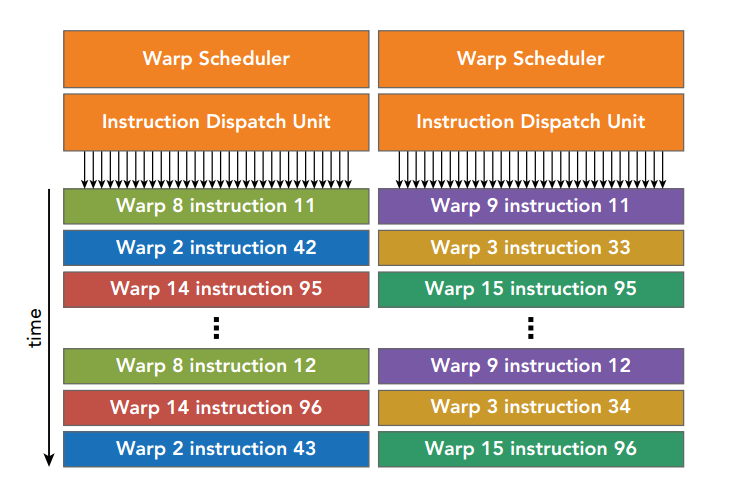
\includegraphics[width=0.9\textwidth]{assets/warp.png}\\
单个SM(Stream Multiprocessor)包括如下组成部分:
\begin{itemize}
	\item Core,也叫流处理器Stream Processor
	\item LD/ST(load/store)模块来加载和存储数据
	\item SFU(Special function units)执行特殊数学运算(sin、cos、log等
	\item 寄存器(Register File)
	\item L1缓存
	\item 全局内存缓存(Uniform Cache)
	\item 纹理缓存(Texture Cache)
\end{itemize}

\subsubsection{逻辑上}
\noindent
\textcolor{blue}{thread hierarchy}\footnote{\href{https://blog.csdn.net/yangjinyi1314/article/details/124905292}{cuda核函数的并行机制}}:\\
grid,block,thread,warp\\
gridDim(blockIdx.x
blockIdx.y,
blockIdx.z),blockDim(threadIdx.x,threadIdx.y,threadIdx.z)\\

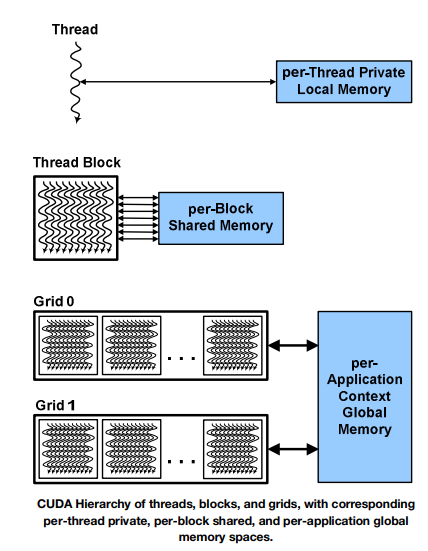
\includegraphics[width=0.9\textwidth]{assets/thread.png}\\
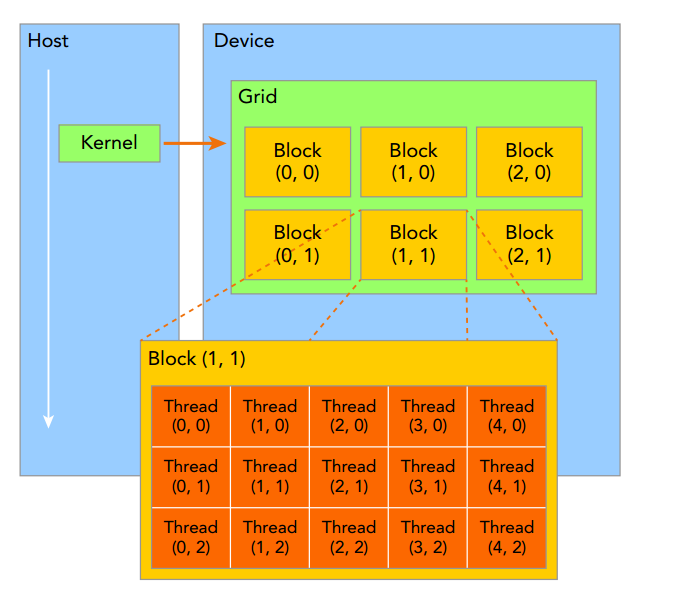
\includegraphics[width=0.9\textwidth]{assets/thread2.png}\\
\textcolor{blue}{memory hierarchy}\footnote{\href{https://blog.csdn.net/xukang95/article/details/102855750}{cuda内存层次}}:\\
register,local memory,shared memory,constant memory,texture memory,global memory,host memory\\
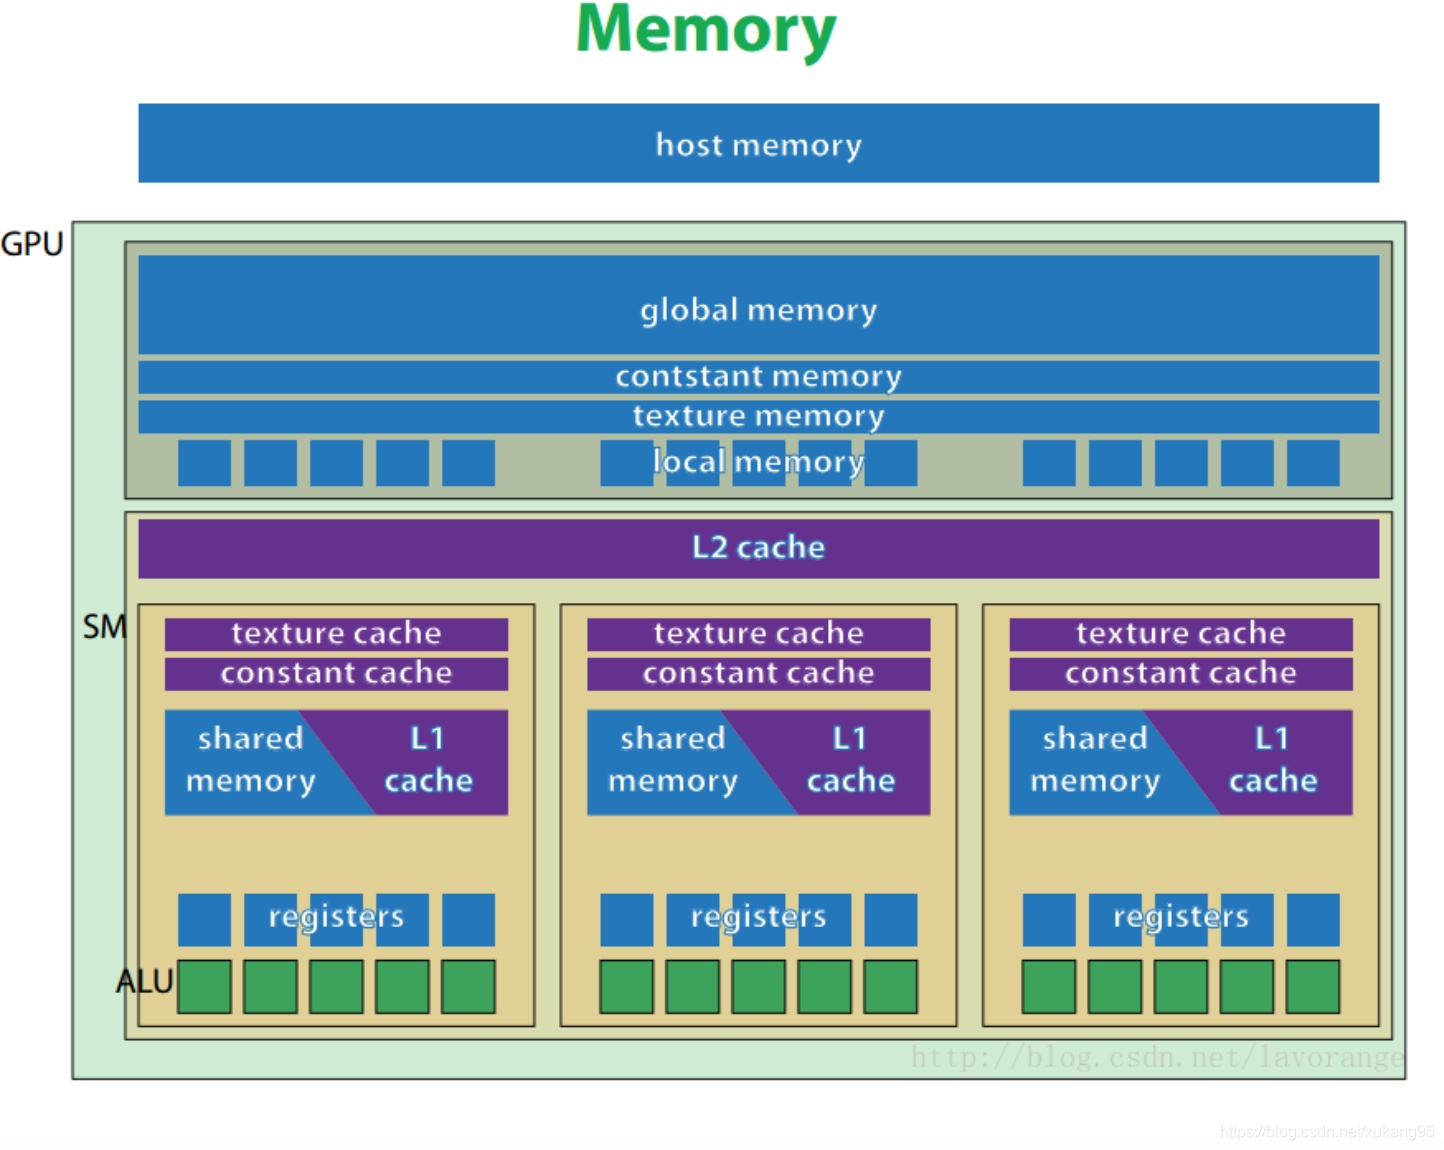
\includegraphics[width=0.9\textwidth]{assets/mem.jpg}\\

\subsubsection{CUDA C}
\noindent
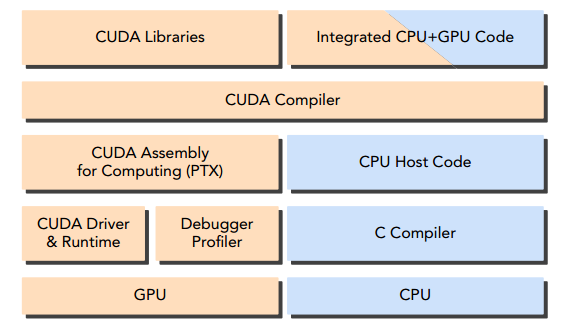
\includegraphics[width=0.9\textwidth]{assets/cudac.png}\\
\textcolor{blue}{nvcc},编译工具\\
\textcolor{blue}{NVIDIA Nsight Compute},ncu
\textcolor{blue}{NVIDIA Nsight Systems},nsys,系统分析工具\\
CUDA C syntax
\subsection{本机实验环境}
\noindent
GPU:NVIDIA GeForce RTX 3050 Laptop GPU\\
Driver Version: 470.141.03   \\
CUDA Version: 11.4\\
nvcc:Cuda compilation tools, release 11.0, V11.0.194

\section{cuda编程练习}
\noindent
(APOD开发模型,即:Assess, Parallelize, Optimize, Deploy)

\subsection{矩阵加法}
\subsubsection{实验结果}
\noindent
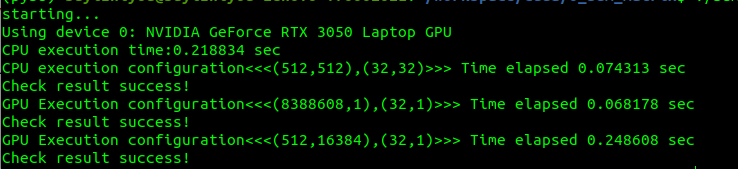
\includegraphics[width=0.9\textwidth]{assets/matrix.png}
\subsubsection{分析总结}
\noindent
不同的execution configuration会影响执行性能,因此尝试不同的grid和block dimensions可能产生更好的性能。

\subsection{warp divergence}
\subsubsection{实验结果}
\noindent
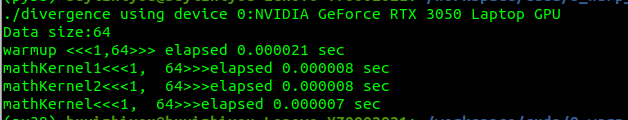
\includegraphics[width=0.9\textwidth]{assets/warp_d.png}
\subsubsection{分析总结}
\noindent
同一个warp内的线程必须执行同一条指令,当线程内存在控制流时,不同线程可能有不同的执行路径,这会降低核函数效率,所以要尽量避免同一个warp内的线程分化。

\subsection{数组求和}
\subsubsection{实验结果}
\noindent
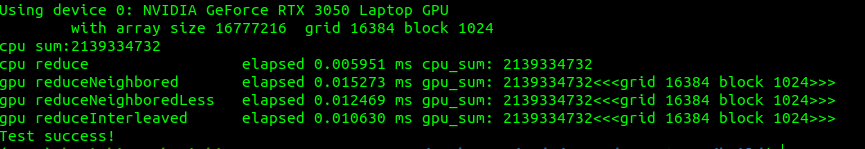
\includegraphics[width=0.9\textwidth]{assets/sum.png}
\subsubsection{分析总结}
\noindent
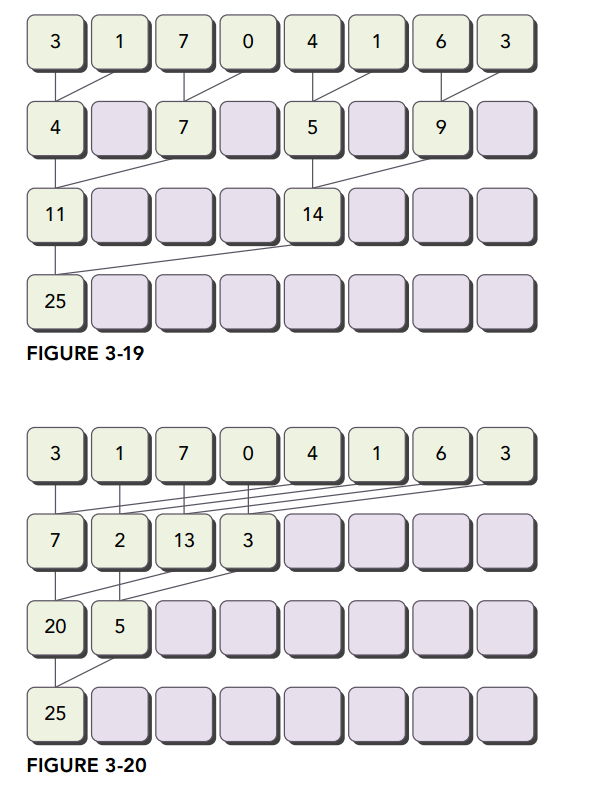
\includegraphics[width=0.9\textwidth]{assets/interleave.png}
\begin{itemize}
	\item The Parallel Reduction Problem(并行规约问题),避免分支分化
	\item 使用interleaved pair approach替代neighbored approach,性能提升,主要原因是global memory加载和存储模式
\end{itemize}


\subsection{循环展开}
\subsubsection{实验结果}
\noindent
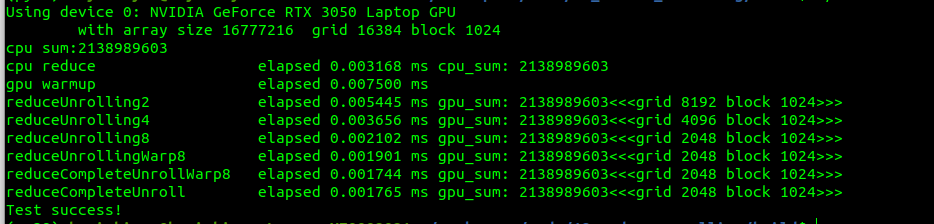
\includegraphics[width=0.9\textwidth]{assets/loop.png}
\subsubsection{分析总结}
\noindent
\begin{itemize}
	\item 循环展开是一种通过减少分支和循环指令来优化程序性能的方法,利用手动重复执行某个操作来代替一个循环体
\end{itemize}


\subsection{结构体数组vs数组结构体}
\subsubsection{实验结果}
\noindent
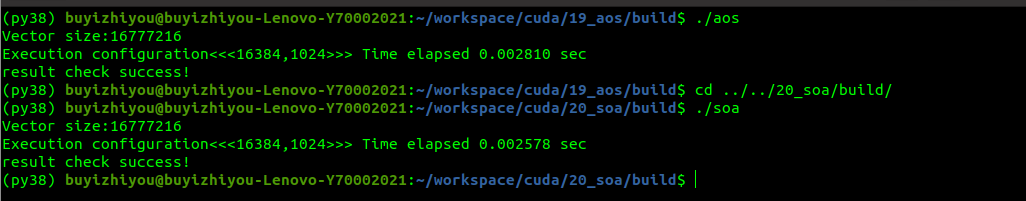
\includegraphics[width=0.9\textwidth]{assets/aos.png}
\subsubsection{分析总结}
\noindent
\begin{itemize}
	\item 并行编程范式,尤其是SIMD(单指令多数据)对SoA更友好。CUDA中普遍倾向于SoA因为这种内存访问可以有效地合并。
\end{itemize}


\subsection{矩阵转置}
\subsubsection{实验结果}
\noindent
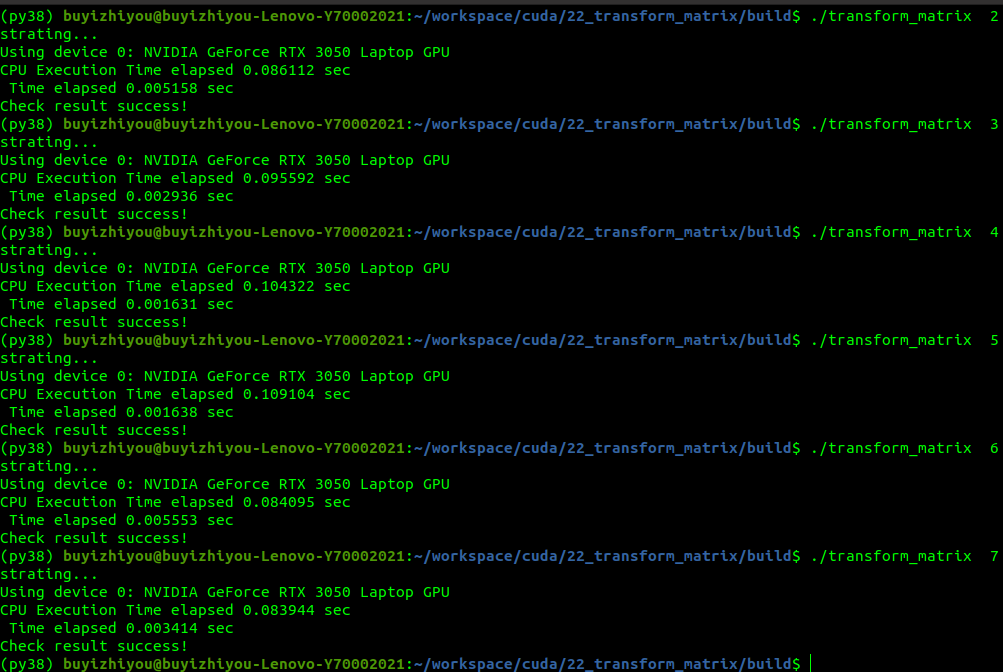
\includegraphics[width=0.9\textwidth]{assets/diag.png}
\subsubsection{分析总结}
\noindent
\begin{itemize}
	\item 2,3分别是按行读取和按列读取,按列读取的吞吐量大于按行读取的原因是缓存命中
	\item 4,5分别是利用循环展开提升性能
	\item 6,7是使用对角化的方式,提高对存储块的均匀访问
\end{itemize}


\subsection{共享内存的读写}
\subsubsection{实验结果}
\noindent
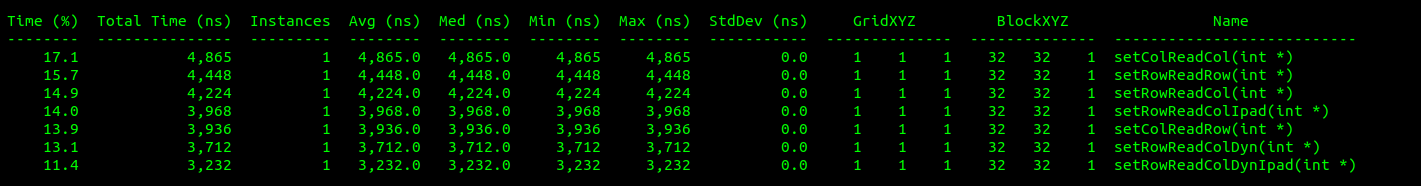
\includegraphics[width=0.9\textwidth]{assets/sm.png}
\subsubsection{分析总结}
\noindent
\begin{itemize}
	\item shared memory的行主序读写和列主序读写,按照行主序读和写,减少共享内存冲突
	\item shared memory的动态分配,在$<<<...>>>$里面可以指定分配的shared memory
	\item shared memory的padding,减少back conflicts
\end{itemize}

\subsection{利用共享内存做reduce求和任务}
\subsubsection{实验结果}
\noindent
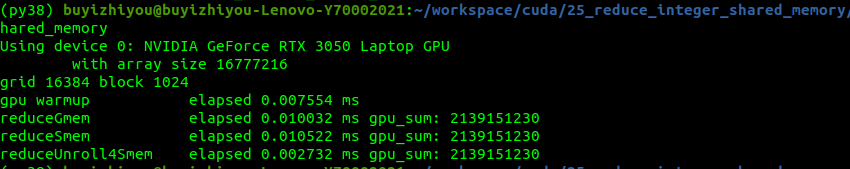
\includegraphics[width=0.9\textwidth]{assets/smem.png}
\subsubsection{分析总结}
\noindent
\begin{itemize}
	\item 可以看到使用shared memory相比使用global memory带来的性能提升。因为shared memory是片上(on-chip),可以减少访问全局内存的时间。
\end{itemize}

\subsection{cuda stream}
\subsubsection{实验结果}
\noindent
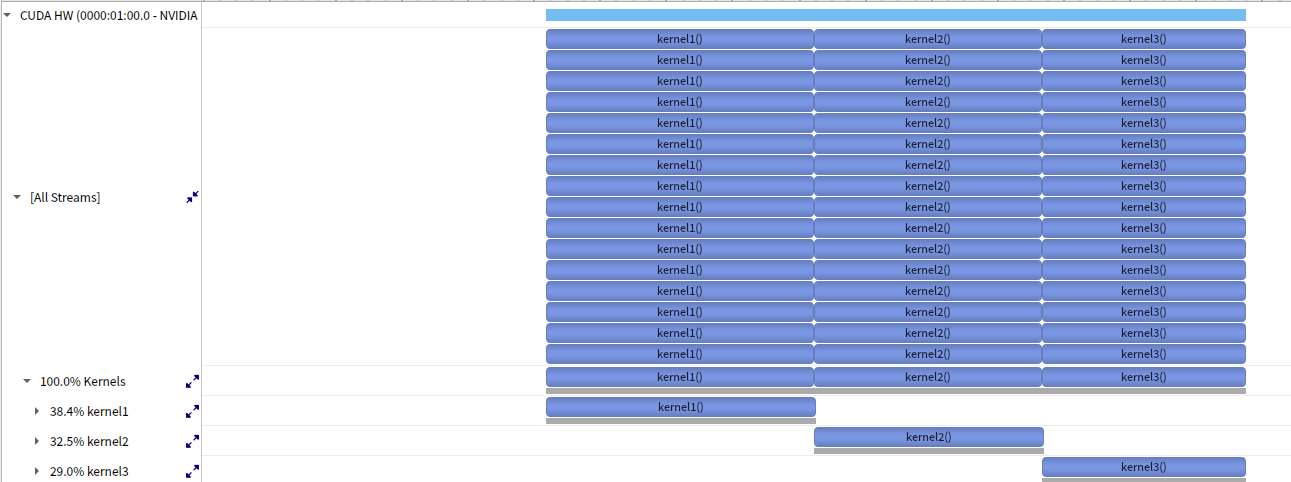
\includegraphics[width=0.9\textwidth]{assets/stream.png}
\subsubsection{分析总结}
\noindent
\begin{itemize}
	\item 可以看到使用shared memory相比使用global memory带来的性能提升。因为shared memory是片上(on-chip),可以减少访问全局内存的时间。
\end{itemize}


\subsection{kernel执行和数据传输重叠}
\subsubsection{实验结果}
\noindent
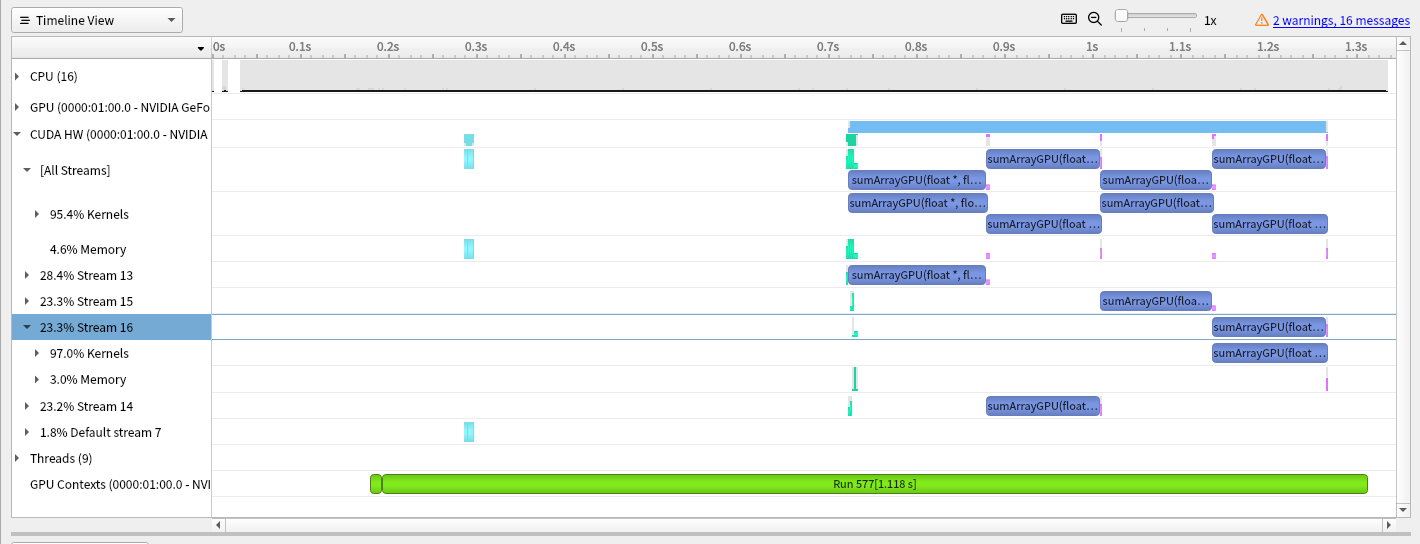
\includegraphics[width=0.9\textwidth]{assets/overlap.png}
\subsubsection{分析总结}
\noindent
\begin{itemize}
	\item 不同流中内核相互重叠,内核执行和数据传输重叠,不同流中不同方向(HtoD or DtoH)的数据传输重叠
	\item 数据传输使用异步方式,注意异步处理的数据要声明称为固定内存
\end{itemize}

\section{总结}
\begin{itemize}
	\item 性能测试命令ncu有问题,没办法做更精确的测试
	\item cuda版本问题
	\item 不同GPU架构有点混乱
\end{itemize}
\section{参考资料}
\noindent
1.《Professional CUDA C Programming》 \\
2. https://face2ai.com/
\end{document}